%%% attributes specified in assignment
\documentclass[11pt, a4paper]{article}
\usepackage[left=2cm, top=3cm, text={17cm, 24cm}]{geometry}
\usepackage{times} %% font times
%%%

%%% my attributes
\usepackage[utf8]{inputenc}
\usepackage[czech]{babel}
\usepackage{multirow}
\usepackage{graphics}
\usepackage{pdflscape}
\usepackage{tikz}
\usetikzlibrary{backgrounds}
\usepackage[linesnumbered, ruled, noline, czech, longend]{algorithm2e}
\usepackage[hidelinks, draft=false]{hyperref}  % hide borders around links
%%%


\begin{document}
	\begin{titlepage}
		\begin{center}
				\Huge{\textsc{Vysoké učení technické v~Brně}}\\
				\huge{\textsc{Fakulta informačních technologií}}
			\\
			\vspace{
			    \stretch{0.382}
			}
			\LARGE{Typografie a publikování\,--\,3. projekt}\\
			\Huge{Tabulky a obrazky}
			\vspace{
			    \stretch{0.618}
			}			
		\end{center}
    	{\Large \today \hfill Samuel Dobroň}
	\end{titlepage}

\section{Úvodní strana}
	Název práce umístěte do zlatého řezu a nezapomeňte uvést \uv{dnešní} datum a vaše jméno a příjmení.

\section{Tabulky}
    Pro sázení tabulek můžeme použít buď prostředí\texttt{ tabbing }nebo prostředí\texttt{ tabular}.

\subsection{Prostředí\texttt{ tabbing}}
    Při použití\texttt{ tabbing }vypadá tabulka následovně: \begin{tabbing}
        Vodní melouny \quad \= 25,90 \quad \= \textbf{Množství} \kill %let longest lines set columns width
        \textbf{Ovoce} \> \textbf{Cena} \> \textbf{Množství} \\
        Jablka  \>  25,90   \>  3\,kg \\
        Hrušky  \>  27,40   \>  2,5\,kg\\
        Vodní melouny \>    35,--  \> 1\,kus\\
    \end{tabbing}
    \noindent Toto prostředí se dá také použít pro sázení algoritmů, ovšem vhodnější je použít prostředí\texttt{ algorithm }nebo \texttt{algorithm2e }(viz sekce \ref{sec:3}).

\subsection{Prostředí\texttt{ tabular}}
    Další možností, jak vytvořit tabulku, je použít prostředí\texttt{ tabular}. Tabulky pak budou vypadat takto\footnote{Kdyby byl problem s\texttt{ cline,} zkuste se podívat třeba sem: http://www.abclinuxu.cz/tex/poradna/show/325037.}
    \catcode`\-=12 \bigskip
        \begin{table}[h]
        \centering
        \begin{tabular}{| l | c | c |}
        \hline
            & \multicolumn{2}{c |}{\textbf{Cena}} \\ \cline{2-3}
            \textbf{Měna}    &   \textbf{nákup}   &   \textbf{prodej} \\
            \hline
            EUR     &   24,775  &   25,943 \\
            GBP     &   29,394  &   30,492 \\
            USD     &   22,423  &   23,661 \\
            \hline
    \end{tabular} \\
    \caption{Tabulka kurzů k~dněšnímu dni}
    \label{table:1}
    \end{table}
    
    \catcode`\-=12 \bigskip
        \begin{table}[h]
        \centering
        \begin{tabular}{cccc}
        \begin{tabular}{| c | c |}
            \hline
            A~&   $\neg$A \\
            \hline
            \textbf{P}  &   N \\
            \hline
            \textbf{O}  &   O~\\
            \hline
            \textbf{X}  &   X \\
            \hline
            \textbf{N}  &   P \\
            \hline
        \end{tabular}
        
        \begin{tabular}{| c | c | c | c | c | c |}           
            \hline
            \multicolumn{2}{| c |}{
                \multirow{2}{*}{$A \wedge B$}
            }
            &
            \multicolumn{4}{| c |}{
                $B$
            }\\ \cline{3-6}
            \multicolumn{2}{| c |}{} & \textbf{P} & \textbf{O} & \textbf{X} & \textbf{N} \\ \hline
            \multirow{4}{*}{
                $A$
            } & \textbf{P} & P & O~& X & N\\ \cline{2-6}
              & \textbf{O} & O~& O~& X & N\\ \cline{2-6}
              & \textbf{X} & X & N & X & N\\ \cline{2-6}
              & \textbf{N} & N & N & X & N\\ \cline{2-6}
            \hline
        \end{tabular}
        
        \begin{tabular}{| c | c | c | c | c | c |}           
            \hline
            \multicolumn{2}{| c |}{
                \multirow{2}{*}{$A \vee B$}
            }
            &
            \multicolumn{4}{| c |}{
                $B$
            }\\ \cline{3-6}
            \multicolumn{2}{| c |}{} & \textbf{P} & \textbf{O} & \textbf{X} & \textbf{N} \\ \hline
            \multirow{4}{*}{
                $A$
            } & \textbf{P} & P & P & P & P\\ \cline{2-6}
              & \textbf{O} & P & O~& P & O\\ \cline{2-6}
              & \textbf{X} & P & P & X & X\\ \cline{2-6}
              & \textbf{N} & P & O~& X & N\\ \cline{2-6}
            \hline
        \end{tabular}
        
        \begin{tabular}{| c | c | c | c | c | c |}           
            \hline
            \multicolumn{2}{| c |}{
                \multirow{2}{*}{$A \rightarrow B$}
            }
            &
            \multicolumn{4}{| c |}{
                $B$
            }\\ \cline{3-6}
            \multicolumn{2}{| c |}{} & \textbf{P} & \textbf{O} & \textbf{X} & \textbf{N} \\ \hline
            \multirow{4}{*}{
                $A$
            } & \textbf{P} & P & O~& X & N\\ \cline{2-6}
              & \textbf{O} & P & O~& P & O\\ \cline{2-6}
              & \textbf{X} & P & P & X & X\\ \cline{2-6}
              & \textbf{N} & P & P & P & P\\ 
            \hline
        \end{tabular}
        \end{tabular}
        \caption{Protože Kleeneho trojhodnotová logika už je \uv{zastaralá}, uvádíme si zde příklad čtyřhodnotové logiky}
        \label{table:2}
        \end{table}
    \bigskip
    \pagebreak

\section{Algoritmy}
\label{sec:3}
    Pokud budeme chtít vysázet algoritmus, můžeme použít prostředí\texttt{ algorithm}\footnote{Pro nápovědu, jak zacházet
s~prostředím\texttt{ algorithm,} můžeme zkusit tuhle stránku:\\ http://ftp.cstug.cz/pub/tex/CTAN/macros/latex/contrib/algorithms/algorithms.pdf.} \quad\!\!nebo\texttt{ algorithm2e}\footnote{Pro\texttt{ algorithm2e }zase tuhle: http://ftp.cstug.cz/pub/tex/CTAN/macros/latex/contrib/algorithm2e/doc/algorithm2e.pdf.}. Příklad použití prostředí\texttt{ algorithm2e }viz Algoritmus \ref{algo}.
    \bigskip
    \IncMargin{1.5em} 
    \begin{algorithm}
        \SetNlSty{textnormal}{}{:}
    \Indm\Indmm
        \KwIn{$(X_{t-1}, u_t, z_t)$}
        \KwOut{$ X_t $}
    \Indp\Indpp
        \BlankLine
    \SetNlSkip{0.3em}
        $\overline{X_t} = X_t = 0$ \\
        \For{$k = 1$ \textnormal{to} $M$}
        {
            $x^{[k]}_t = \emph{sample\_motion\_model}(u_t, x^{[k]}_{t-1})$ \\
            $\omega^{[k]}_t = \emph{measurement\_model}(z_t, x^{[k]}_t, m_{t-1})$ \\
            $m^{[k]}_t = updated\_occupancy\_grid(z_t, x^{[k]}_t, m^{[k]}_{t-1})$ \\
            $\overline{X_t} = \overline{X_t} + \langle x^{[m]_x}, \omega^{[m]}_t \rangle$
        }
        \For{$k = 1$ \textnormal{to} $M$}
        {
            draw $i$ with probability $\approx \omega^{[i]}_t$ \\
            add $\langle x^{[k]}_x, m^{[k]}_t \rangle$ to $X_t$ \\
        }
        \KwRet{$X_t$}
    \caption{\textsc{FastSLAM}}
    \label{algo}
    \end{algorithm}
    \vspace{-0.566em}
    
\section{Obrázky}
    Do našich članků můžeme samozřejmě vkládat obrázky. Pokud je obrázkem fotografie, můžeme klidně použít bitmapový soubor. Pokud by to ale mělo být nejaké schéma nebo něco podobného, je dobrým zvykem takovýto obrázek vytvořit vektorově.
    \begin{figure}[h]
    \begin{center}
    \scalebox{0.4}{
        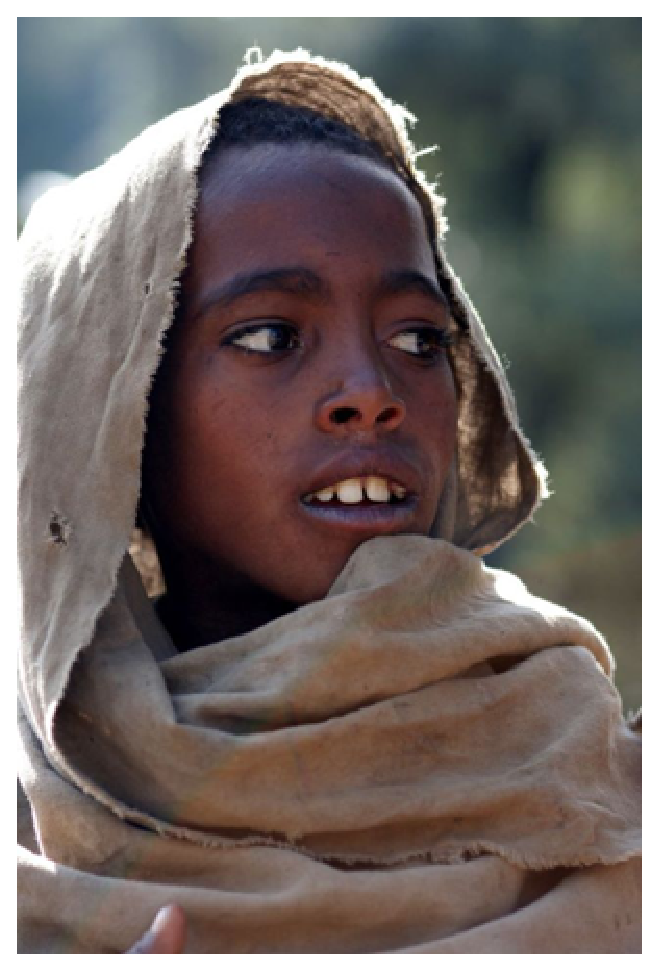
\includegraphics{etiopan.eps}
        \reflectbox{
            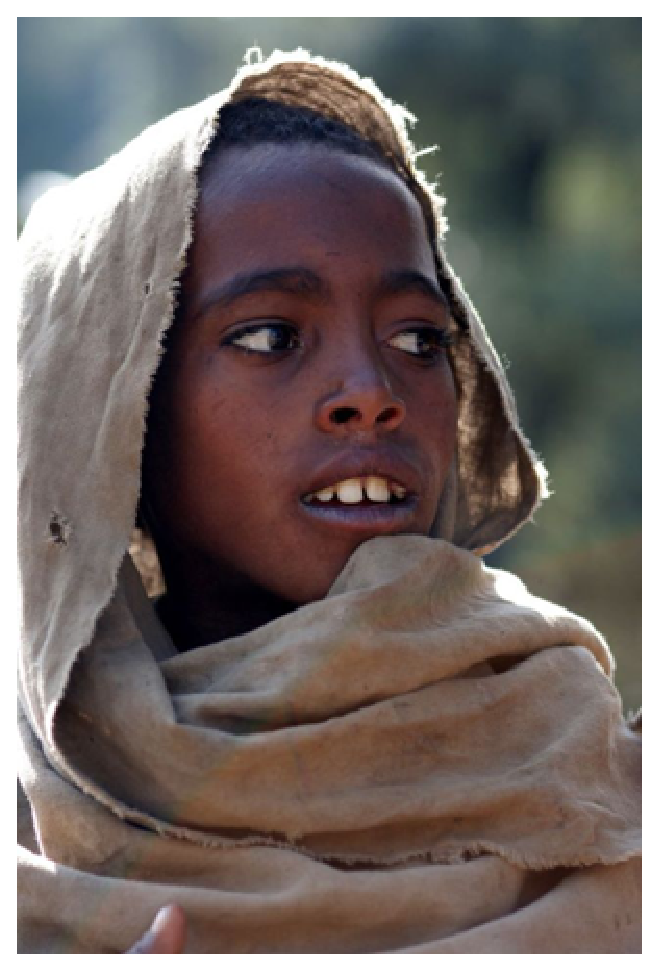
\includegraphics{etiopan.eps}
        }
        
    }
    \caption{Malý Etiopánek a jeho bratříček}
    \label{etiopan}
    \end{center}
    \end{figure}
    \pagebreak
    
    Rozdíl mezi vektorovým \dots
    \begin{figure}[h]
        \begin{center}
        \scalebox{0.4}{
            
\includegraphics{oniisan.eps}
        }
        \caption{Vektorový obrázek}
        \label{onisan}
        \end{center}
    \end{figure}
    
    \noindent \dots a bitmapovým obrázkem
    \begin{figure}[h]
        \begin{center}
        \scalebox{0.6}{
           
\includegraphics{oniisan2.eps}
        }
        \caption{Bitmapový obrázek}
        \label{onisan2}
        \end{center}
    \end{figure}
    
    \noindent se projeví například při zvětšení.
    
    Odkazy (nejen ty) na obrázky \ref*{etiopan}, \ref*{onisan} a \ref*{onisan2}, na tabulky \ref*{table:1} a \ref*{table:2} a také na algoritmus \ref*{algo} jsou udělány pomocí křížových odkazů. Pak je ovšem potřeba zdrojový soubor přeložit dvakrát.
    
    Vektorové obrázky lze vytvořit i přímo v~\LaTeX{u}, například pomocí prostředí\texttt{ picture} .
    
% House
    \begin{landscape}
        \begin{figure}[ht]
            \begin{center}
            \label{image:dom}
            \begin{tikzpicture}[framed]
                %%left part
                \draw[thick,rounded corners=4pt]
                    (0,0) -- (0,6) -- (3, 8.9);
                \draw[thick, rounded corners=4pt]
                    (0.2, 0) -- (0.2, 5.9) -- (3, 8.6);
                \draw[thick]
                    (3, 3) -- (0.2, 2.3);
                \draw[thick]
                    (3, 6.6) -- (0.2, 5.8);
                \draw[thick]
                    (0.5, 5.7) -- (2.6, 6.3) -- (2.6, 4.9) -- (0.5, 4.4) -- (0.5, 5.7);
                \draw[thick]
                    (0.5, 2.2) -- (2.6, 2.7) -- (2.6, 1.5) -- (0.5, 1.1) -- (0.5, 2.2);
                    
                %%% tube
                \draw
                    (3,9) .. controls (3.5,9.5) and (5.5, 9.5) .. (6,9);
                \draw[thick,rounded corners=4pt]
                    (3,9) -- (3, 0);
                \draw[thick,rounded corners=4pt]
                    (6, 5.7) -- (6, 0);
                \draw
                    (3,0) .. controls (3.5, -0.5) and (5.5, -0.5) .. (6, 0);
                \draw
                    (3, 3) .. controls (3.5, 2.8) and (5.5, 2.8) .. (6, 3);
                \draw
                    (3,6.6) .. controls (3.5, 7) and (5.5, 7) .. (6, 6.5);
                
                %%right part
                \draw[thick, rounded corners=4pt]
                    (6,9) -- (6, 5.5) -- (10, 4) -- (10, -0.5);
                \draw[thick, rounded corners=2pt]
                    (6.5, 1) -- (8, 1) -- (8, 4) -- (6.5, 4.5) -- (6.5, 1);
                \draw[thick]
                    (8.8, -0.5) -- (8.8, 1.2) -- (9.5, 1) -- (9.5, -0.5);
                
                %%ground
                \draw[ultra thick]
                    (-2, 0) -- (2.8, 0) -- (2.3, -.5) -- (12, -.5) -- (12, -0.7) -- (1.9, -0.7) -- (2.4, -0.2) -- (-2, -0.2) -- (-2, 0);
                    
                %%water
                \draw[thick, draw=blue]
                    (0, -2) .. controls (0.2, -1.5) and (0.8, -2.5) .. (1, -2);
                \draw[thick, draw=blue]
                    (3, -2.3) .. controls (3.2, -1.8) and (3.8, -2.8) .. (4, -2.3);
                \draw[thick, draw=blue]
                    (7, -2.3) .. controls (7.2, -1.8) and (7.8, -2.8) .. (8, -2.3);
                \draw[thick, draw=blue]
                    (9, -3.3) .. controls (9.2, -2.8) and (9.8, -3.8) .. (10, -3.3);
                \draw[thick, draw=blue]
                    (0, -3.3) .. controls (0.2, -2.8) and (1.3, -2.8) .. (1.5, -3.3);
                \draw[thick, draw=blue]
                    (5, -3.3) .. controls (5.2, -2.8) and (6.3, -2.8) .. (6.5, -3.3);
                
                %sun
                \filldraw[thick, color=yellow, fill=yellow!5,] (10, 10) circle(1);
            \end{tikzpicture}
            \caption{Vektorový obrázek moderního bydlení vhodného pro 21. století.}
             \end{center}
        \end{figure}
    \end{landscape}
\end{document}
